% Created 2023-08-24 木 16:48
% Intended LaTeX compiler: pdflatex
\documentclass[10pt]{article}
\usepackage[utf8]{inputenc}
\usepackage[T1]{fontenc}
\usepackage{graphicx}
\usepackage{longtable}
\usepackage{wrapfig}
\usepackage{rotating}
\usepackage[normalem]{ulem}
\usepackage{amsmath}
\usepackage{amssymb}
\usepackage{capt-of}
\usepackage{hyperref}
\usepackage[newfloat]{minted}
\usepackage[a4paper, total={6.5in, 9in}]{geometry}
\usepackage{minted}
\setminted{breaklines}
\usepackage[utf8]{inputenc}
\renewcommand{\familydefault}{\sfdefault}
\usemintedstyle{vs}
\usepackage{CJKutf8}
\usepackage{xurl}
\usepackage{fontawesome5}
\usepackage{hyperref}
\usepackage{graphicx}
\usepackage{float}
\newcommand{\gitlab}[1]{%
\href{#1}{GitLab \faGitlab}}
\author{Vincent Conus}
\date{2023-8-24}
\title{Setting up and using Xilinx KRIA KV260\\\medskip
\large \begin{CJK}{UTF8}{min}南山大学\end{CJK}}
\hypersetup{
 pdfauthor={Vincent Conus},
 pdftitle={Setting up and using Xilinx KRIA KV260},
 pdfkeywords={},
 pdfsubject={A report presenting how to use and set Xilinx's Kria board},
 pdfcreator={Emacs 30.0.50 (Org mode 9.6.6)}, 
 pdflang={English}}
\begin{document}

\begin{titlepage}
\centering
{\LARGE Setting up and using Xilinx KRIA KV260 \par }
\vspace{5mm}
{\large \begin{CJK}{UTF8}{min}南山大学\end{CJK} \par}
\vspace{2cm}
{\large Vincent Conus -  Source available at \gitlab{https://gitlab.com/sunoc/xilinx-kria-kv260-documentation} \par}
\vspace{3cm}
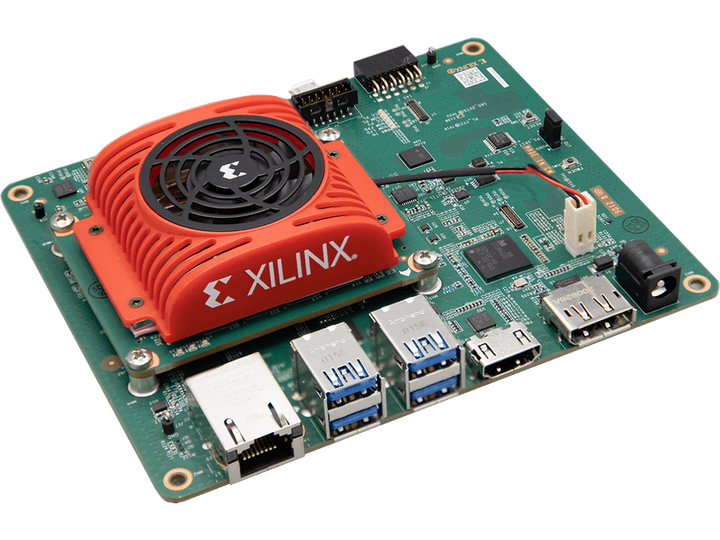
\includegraphics[width=0.8\textwidth]{./img/board}\end{titlepage}
\tableofcontents
\pagebreak
\section{Introduction}
\label{sec:orgb4c4546}
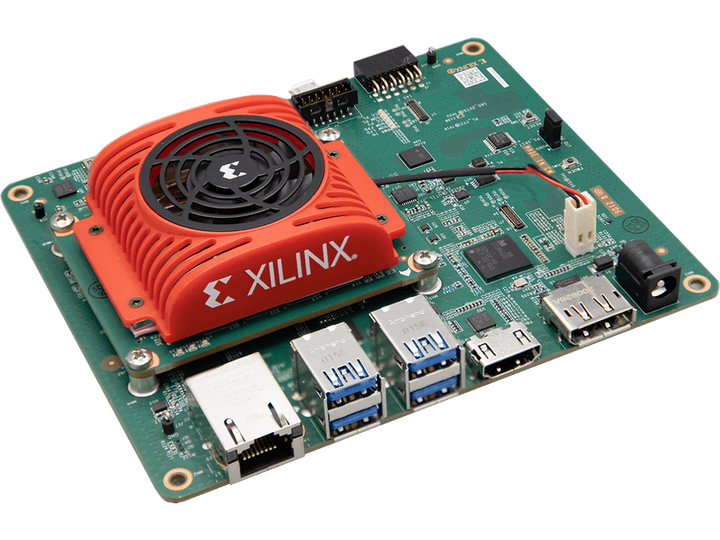
\includegraphics[width=0.8\textwidth]{./img/board.png}

\section{Build instructions}
\label{sec:org75a877d}
On a moderately recent Ubuntu-base distribution, the following packages seemed to be required to build the
report:

\begin{minted}[frame=single,framesep=2mm,baselinestretch=1.2,linenos,breaklines,fontsize=\footnotesize]{bash}
sudo apt-get install texlive-base texlive-latex-recommended texlive-lang-japanese
\end{minted}

Then, the actual build can be made with a simple:

\begin{minted}[frame=single,framesep=2mm,baselinestretch=1.2,linenos,breaklines,fontsize=\footnotesize]{bash}
pdflatex instructions.tex
\end{minted}

No fancy Lua or theme at the moment !

\section{Automatic build with CI/CD pipeline}
\label{sec:orgd342161}
If you don't want to build the report yourself, a CI pipeline is used to make it on GitLab.

You can check the steps in the .gitlab-ci.yml file.
This build uses a base Ubuntu image and basically takes the same steps as presented above for a local build.

A PDF artifact can be downloaded.
\end{document}